% !TeX root = ../../main.tex
% Add the above to each chapter to make compiling the PDF easier in some editors.


% recently published  \cite{Xu16-InteractiveObjectSelection} \cite{JG18-ClickCarving} \cite{Liew17-RegionalInteractiveImageSeg}

%%% Motivation
% Fast development in computer science -> ML and automation of processes in the industry.
The development in machine vision has continued to make great strides in recent years. 
For this thesis two areas are emphasized in particular: \gls{ml} and the automation of industrial processes.
The former is driven by an energetic research community, resulting in novel methods and application areas.
% Increasing automation == increasing application of image processing (-> application of DL).
The latter enjoys the benefits of increasing digitization and the developments in hardware, computational power, and image processing due to \gls{ml}.


% Semantic Segmentation of Images as valueable method with increasing application.
A widely used method in image processing is semantic segmentation, that performs pixel-wise classification.
Segmentation is a valuable instrument, in order to identify and pixel-precise localize objects in images.
Recently, segmentation methods based on \gls{dl} emerged, resulting in advanced performance in the form of higher accuracy and richer detail.
A popular application is the automation of repetitive processes in industrial manufacturing with as the detection of errors, the counting of instances or the control of quality \cite{Rah19-IoT} \cite{Chen19-AnomalyDetectionManufacturing}.

One advantage of using segmentation methods is the pixel-precise prediction, which provides many detail on the object as presented in Figure \ref{fig:ch1:image_industrial}.
On the other side a drawback is the requirement of images with pixel-precise labels, which are expensive to create.
\begin{figure} [b]
	\centering
	\begin{subfigure}[b]{0.4\textwidth}
		\centering
		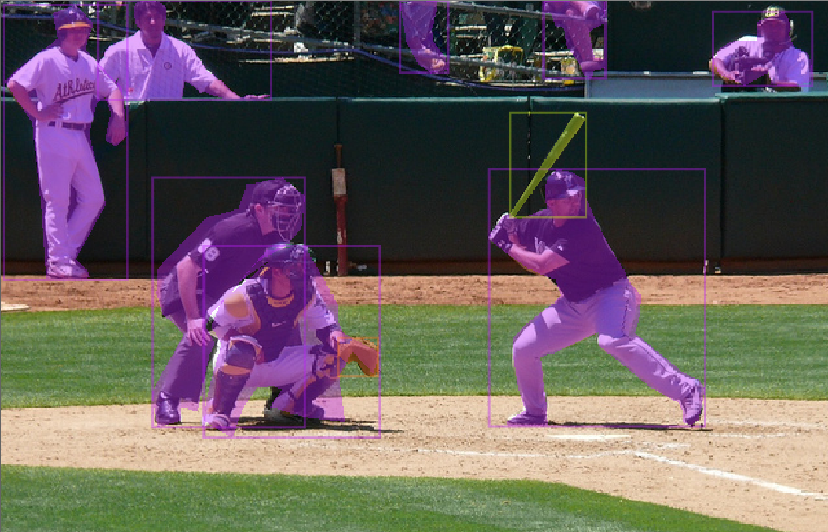
\includegraphics[width=\textwidth]{figures/chap1_general_objects.png}
		\caption{
			Image a of baseball game as example of a general scene.}
		\label{fig:ch1:image_standards}
	\end{subfigure}
	\hfill
	\begin{subfigure}[b]{0.4\textwidth}
		\centering
		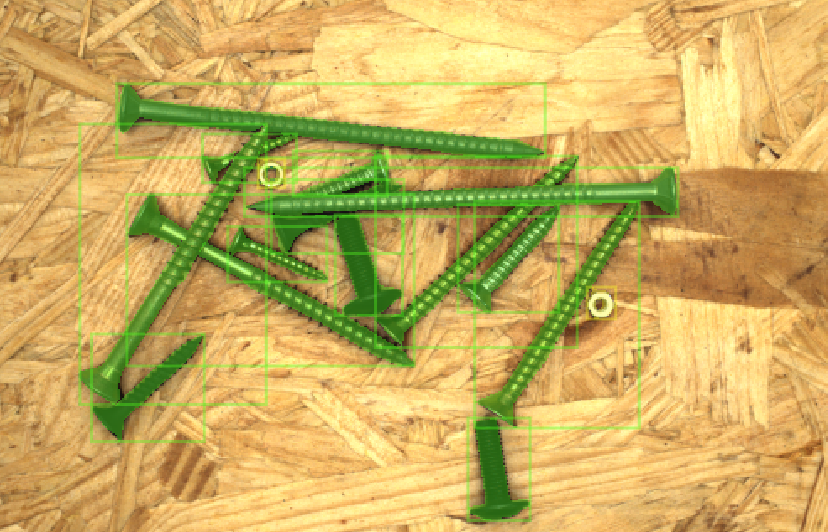
\includegraphics[width=\textwidth]{figures/chap1_industrial_objects.png}
		\caption{
			Image of screws and nuts from an industrial context.}
		\label{fig:ch1:image_industrial}
	\end{subfigure}
	\caption[Semantic Segmentation Visualization]{
		Illustration of the differences between two diverse image domains.
	} \label{fig:ch1:image}
\end{figure}


% -> Interactive Semantic Segmentation 
However, it is possible to extend semantic segmentation by including user interaction, this is referred to as interactive segmentation and may be used to support the label process and create new annotations. 
Thereby, the user interaction often is realized by mouse clicks on the object of interest.
% Use cases for interactive methods
In \cite{Man18-DEXTR} it has already been investigated whether if annotations created by interactive segmentation methods are suitable as \gls{gt} in order to train a new \gls{dl} model.

% Importance of strong generalization capabilities.
In order to be widely used, interactive segmentation methods must have good generalization capabilities with respect to different image domains and different users.
A good generalization over many image domains is important, because when applying these methods often images are used, that are from rather uncommon or unknown domains.
To avoid frequent retaining and allow a constant quality of the created labels, interactive methods should perform equivalent on various domains.
Further, the user of the interactive method is an important factor.
Since users also have different behaviors when using the methods, this can influence the performance of the method.
To prevent this, methods should also have good generalization capabilities over different users.
In current research papers the generalization over various users is hardly investigated, because simulations are mostly used, in order to evaluate the method's performance.

Within the scope of this thesis a benchmark study is performed, that evaluates the application from multiple interactive methods by real users. 
Therefore, realistic insights may be obtained with regard to the generalization capabilities over various user.
This benchmark study is performed on a hand-selected dataset with many different images, to thereby also examine the generalization over various domains.
\\
\newline
%%% Scope of this thesis
This thesis gives an overview of interactive methods for semantic segmentation and evaluates the abilities of specific methods in detail.
In Chapter \ref{ord:ch2} basic types of interactive segmentation methods are presented.
Chapter \ref{ord:ch3} presents the four interactive methods to be evaluated polygond drawing as baseline, watershed transformation, and two state-of-the-art methods based on \gls{dl}: \gls{dextr} and \gls{iog}.
In Chapter \ref{ord:ch4} the benchmark study is presented in detail, which is the core of this thesis.
The special benefit of this benchmark study is the evaluation of real user data in order to examine the method's generalization capabilities over various image domains and users.
The results from the benchmark study are evaluated in Chapter \ref{ord:ch5}.
Here it is examined to what extend interactive segmentation methods based on \gls{ml} improve the process of labeling based on the annotation time and accuracy.
A focus is placed on the generalization capabilities of the methods, which are fundamental for a successful application.
It is also investigated whether annotations created by interactive segmentation models are suitable to be used as training data to train a new \gls{ml} model.
Last, a final conclusion over the results of the benchmark study and the performance of the methods is provided in Chapter \ref{ord:ch6}.

